% Figure 1.3: D₃(n) Pattern for n = 1 to 27
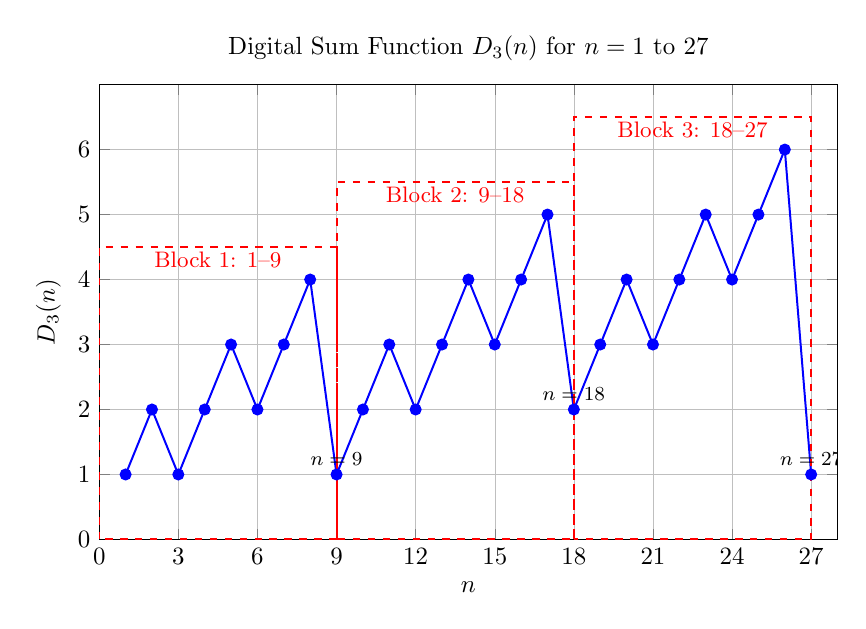
\begin{tikzpicture}[scale=0.9]
\begin{axis}[
    width=12cm,
    height=8cm,
    xlabel={$n$},
    ylabel={$D_3(n)$},
    title={Digital Sum Function $D_3(n)$ for $n = 1$ to $27$},
    xmin=0, xmax=28,
    ymin=0, ymax=7,
    xtick={0,3,6,9,12,15,18,21,24,27},
    ytick={0,1,2,3,4,5,6},
    grid=both,
    grid style={line width=.1pt, draw=gray!10},
    major grid style={line width=.2pt,draw=gray!50},
    legend pos=north west,
]

% Data points for D₃(n)
% n=1: 1, n=2: 2, n=3: 1, n=4: 1+1=2, n=5: 1+2=3, n=6: 2+0=2, n=7: 2+1=3, n=8: 2+2=4, n=9: 1
% n=10: 1+0+1=2, n=11: 1+0+2=3, n=12: 1+1+0=2, n=13: 1+1+1=3, etc.

\addplot[
    color=blue,
    mark=*,
    mark size=2pt,
    thick
] coordinates {
(1,1) (2,2) (3,1) (4,2) (5,3) (6,2) (7,3) (8,4) (9,1)
(10,2) (11,3) (12,2) (13,3) (14,4) (15,3) (16,4) (17,5) (18,2)
(19,3) (20,4) (21,3) (22,4) (23,5) (24,4) (25,5) (26,6) (27,1)
};

% Highlight the repeating pattern blocks
\draw[red, thick, dashed] (axis cs:0,0) rectangle (axis cs:9,4.5);
\node[red, font=\small] at (axis cs:4.5,4.3) {Block 1: 1--9};

\draw[red, thick, dashed] (axis cs:9,0) rectangle (axis cs:18,5.5);
\node[red, font=\small] at (axis cs:13.5,5.3) {Block 2: 9--18};

\draw[red, thick, dashed] (axis cs:18,0) rectangle (axis cs:27,6.5);
\node[red, font=\small] at (axis cs:22.5,6.3) {Block 3: 18--27};

% Annotate special points
\node[above, font=\footnotesize] at (axis cs:9,1) {$n=9$};
\node[above, font=\footnotesize] at (axis cs:18,2) {$n=18$};
\node[above, font=\footnotesize] at (axis cs:27,1) {$n=27$};

\end{axis}
\end{tikzpicture}
